\chapter{Misurazioni e risultati}

\section{Tx\_Cx}
Si vuole simulare un ambiente in cui un nodo, facente le funzioni di server, vuole trasmettere un flusso di pacchetti verso un altro nodo che agirà come un client. 
Nei casi di test che successivamente saranno analizzati, i quattro dispositivi Rock che compongono il testbed verranno suddivisi in due gruppi separati, due in uno e i restanti due in un altro, ognuno con una funzione specifica.

I due gruppi saranno:

\begin{itemize}
    \item \textit{Gruppo Cx}: esso sarà composto da due dispositivi che simuleranno, con modalità che verranno discusse a breve, un ambiente in cui sono presenti uno svariato numero di veicoli che portano il canale di trasmissione a congestionarsi, in maniera completa o parziale.
    \item \textit{Gruppo Tx}: esso, invece, sarà composto da due dispositivi che comunicheranno mediante due flussi TCP in parallelo. Uno di essi agirà come client, che andrà a connettersi e a scaricare delle informazioni dall'altro che fungerà da server.
\end{itemize}

\begin{figure}[h!]
    \centering
    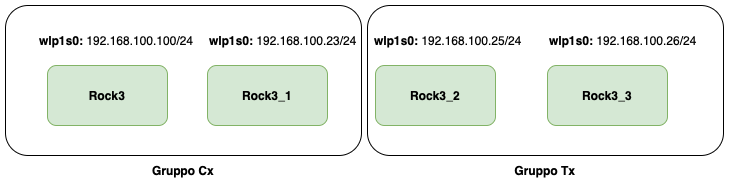
\includegraphics[width=1\textwidth]{diagramma_test.png}
    \caption{Diagramma dispositivi Rock}
    \label{fig:diagramma}
\end{figure}

Sono previsti tre principali casi di test:

\begin{itemize}
    \item \textit{T1\_C0}: assenza di QoS nei flussi dei dispositivi del \textit{Gruppo Tx} e assenza di congestione del canale, quindi il \textit{Gruppo Cx} sarà spento.
    \item \textit{T1\_C1}: assenza di QoS nei flussi dei dispositivi del \textit{Gruppo Tx} e parziale congestione del canale, attuata mediante l'invio in broadcast di CAM da ognuno dei due dispositivi facenti parte del \textit{Gruppo Cx} ogni 5 ms.
    \item \textit{T1\_C2}: assenza di QoS nei flussi dei dispositivi del \textit{Gruppo Tx} e totale congestione del canale, attuata mediante trasmissione UDP in \textit{flooding} in broadcast da parte di ognuno dei due dispositivi del \textit{Gruppo Cx}.
\end{itemize}

Questi stessi casi verranno, inoltre, ripetuti andando ad applicare delle politiche di QoS: un flusso verrà assegnato alla categoria con priorità maggiore, ovvero \textit{Access Category Voice} (AC\_VO), mentre l'altro alla categoria minore, ovvero \textit{Access Category Background} (AC\_BK).

Per fare ciò, viene utilizzato il comando iPerf, già precedentemente discusso, con i dovuti parametri. Nella fattispecie:

\begin{itemize}
    \item \textit{Rock Server}: \verb|iperf -s -i 1 -w 416K -y C -o output.csv|.
    \item \textit{Rock Client - flusso 1}: \\\verb|iperf -c 192.168.100.xxx -t 30 -b 10m -A VO| per il flusso a priorità maggiore.
    \item \textit{Rock Client - flusso 2}: \\\verb|iperf -c 192.168.100.xxx -t 30 -b 10m -A BK| per il flusso a priorità minore.
\end{itemize}

L'indirizzo IP usato nei due comandi è relativo a quello appartenente all'interfaccia \textit{wlp1s0} del dispositivo facente funzione di server.

Nei casi senza politiche di QoS sono stati utilizzati i medesimi comandi, senza ovviamente i parametri che delineano le varie priorità.

Per quanto concerne il raggiungimento di un eventuale congestione del canale, essa è stata raggiunta nei seguenti modi:

\begin{itemize}
    \item \textit{Caso senza congestione}: i dispositivi appartenenti al \textit{Gruppo Cx} non trasmettono alcunchè.
    \item \textit{Caso con congestione parziale}: i dispositivi appartenenti al \textit{Gruppo Cx}, come già detto poc'anzi, trasmettono ognuno un singolo pacchetto CAM ogni 5 ms; per tale scopo è stato lanciato sia su uno che sull'altro Rock lo script riportato in \autoref{udp_packets} con, come parametri, un \textit{message\_size} pari a 256 byte e lo \textit{sleep\_time} pari a 0.005; è stata scelto questo intervallo di tempo in quanto, tenendo conto che in caso di veicolo fermo esso invierebbe un CAM ogni 1 secondo, viene simulato un ambiente con 200 veicoli presenti.
    \item \textit{Caso con congestione totale}: i dispositivi appartenenti al \textit{Gruppo Cx} fanno flooding UDP mediante l'esecuzione del comando \verb|iperf -u -c 192.168.100.xxx| \verb| -t 300 -b 10m|; in questo caso si vuole simulare un ambiente con un numero veramente elevato di veicoli e molto maggiore del caso precedente.
\end{itemize}

In quest'ultimo caso, a causa delle limitazioni architetturali di iPerf, non è stato possibile inviare pacchetti UDP in broadcast. Poiché solo due dispositivi sono incaricati di effettuare flooding, la congestione viene raggiunta trasmettendo messaggi UDP da un dispositivo del \textit{Gruppo Cx} all'altro, specificando come parametro per iPerf l'indirizzo IP dell'interfaccia \textit{wlp1so} del Rock destinatario.

La scelta del protocollo UDP per effettuare \textit{flooding}, anzichè il TCP, è stata effettuata per ovvie ragioni: mancanza di politiche riguardanti il controllo di flusso, perdita dei pacchetti e controllo sull'ordine di ricezione di quest'ultimi. Inoltre, l'invio di essi con una dimensione inferiore a 2346 byte (iPerf, di default, invia pacchetti UDP di soli 1470 byte a differenza del TCP che hanno una dimensione pari a 8 KB \cite{iperf}), consente alle interfacce Wireless di poter trasmettere i vari frame senza attuare il meccanismo di RTS/CTS.

In conclusione, per ogni simulazione sono state effettuati 5 \textit{run} distinti, ciascuno della durata di 30 secondi. Questa scelta è stata fatta per ottenere risultati il più affidabili possibile, escludendo la parte iniziale dell'handshake del protocollo TCP, che potrebbe influenzare i valori iniziali in modo non desiderato.

Verranno, ora, mostrati i risultati ottenuti mediante dei grafici per ogni singolo caso di studio:

\begin{itemize}
    \item il primo mostrerà l'andamento del throughput medio nel corso della simulazione;
    \item il secondo consisterà nel \textit{plot} del throughput di ogni singola \textit{run};
    \item il terzo visualizzerà il carico del canale per tutta la durata della simulazione, inclusi alcuni istanti primae e dopo in modo da mostrare le condizioni iniziali.
\end{itemize}

\noindent Alla fine verranno fatte le dovute considerazioni del caso.

\subsection[QoS assente e congestione assente]{QoS assente e congestione assente}
L'assenza di politiche di QoS, unito ad un canale quasi completamente vuoto e libero da trasmissioni (Figura \ref{fig:t1_c0_load}), porta il throughput di ambedue i flussi ad essere simile al netto di una differenza trascurabile (Tabella \ref{table:6}). Sul canale è possibile trasmettere sino ad un massimo di 10 Mbps teorici, quindi si può tranquillamente notare che le due trasmissioni si suddividono equamente la banda disponibile (Figure \ref{fig:t1_c0} e \ref{fig:t1_c0_ensemble}).

\begin{table}[h!]
    \centering
    \begin{tabular}{|>{\centering\arraybackslash}p{20em}|>{\centering\arraybackslash}p{7em}|} 
     \hline
     \textbf{} & \textbf{Valori} \\ 
     \hline
     \textbf{Throughput Medio per Stream ID 1} & 3.49 Mbps \\ 
     \hline
     \textbf{Throughput Medio per Stream ID 2} & 3.47 Mbps \\
     \hline
    \end{tabular}
    \caption{Valori medi caso QoS assente e congestione assente}
    \label{table:6}
\end{table}

\begin{figure}[h!]
    \centering
    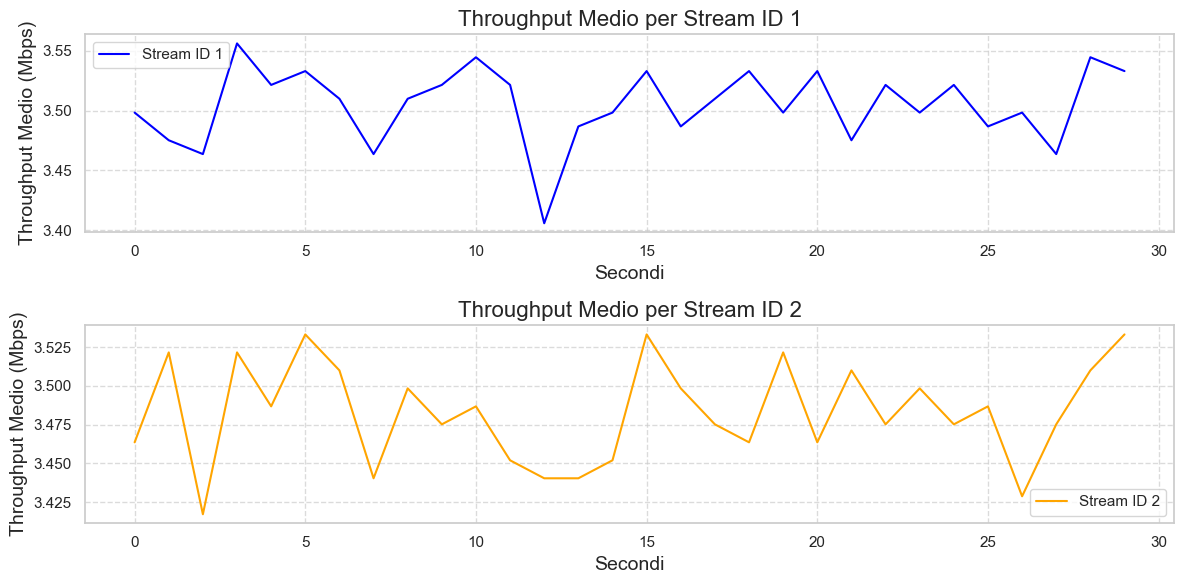
\includegraphics[width=1\textwidth]{t1_c0.png}
    \caption{QoS assente e congestione assente (Throughput medio)}
    \label{fig:t1_c0}
\end{figure}

\begin{figure}[h!]
    \centering
    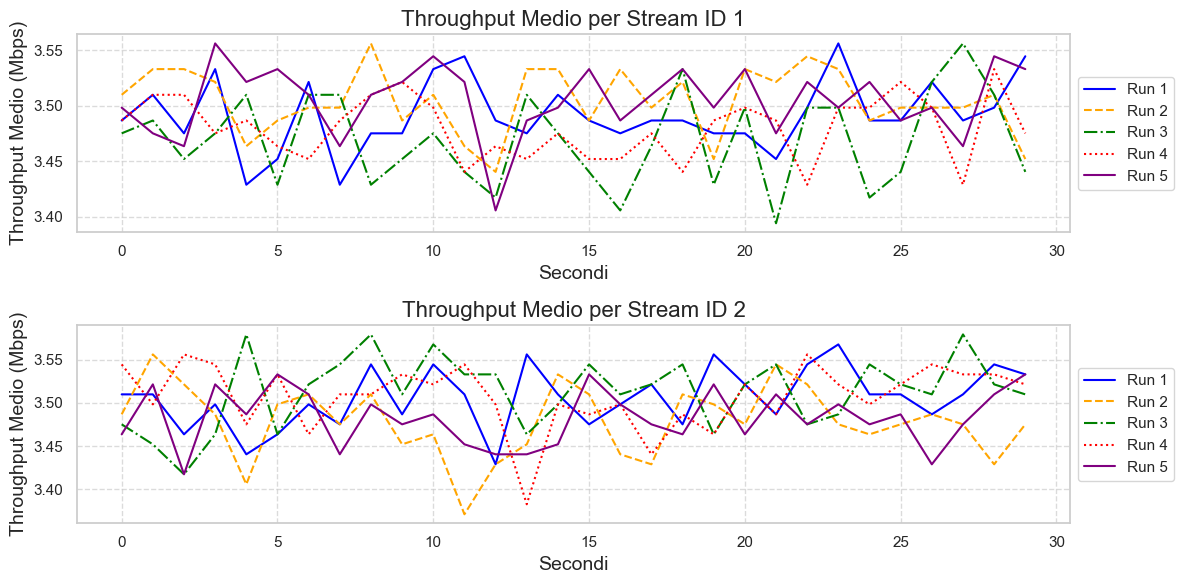
\includegraphics[width=1\textwidth]{t1_c0_ensemble.png}
    \caption{QoS assente e congestione assente (Grafico ensemble)}
    \label{fig:t1_c0_ensemble}
\end{figure}
\clearpage
\begin{figure}[h!]
    \centering
    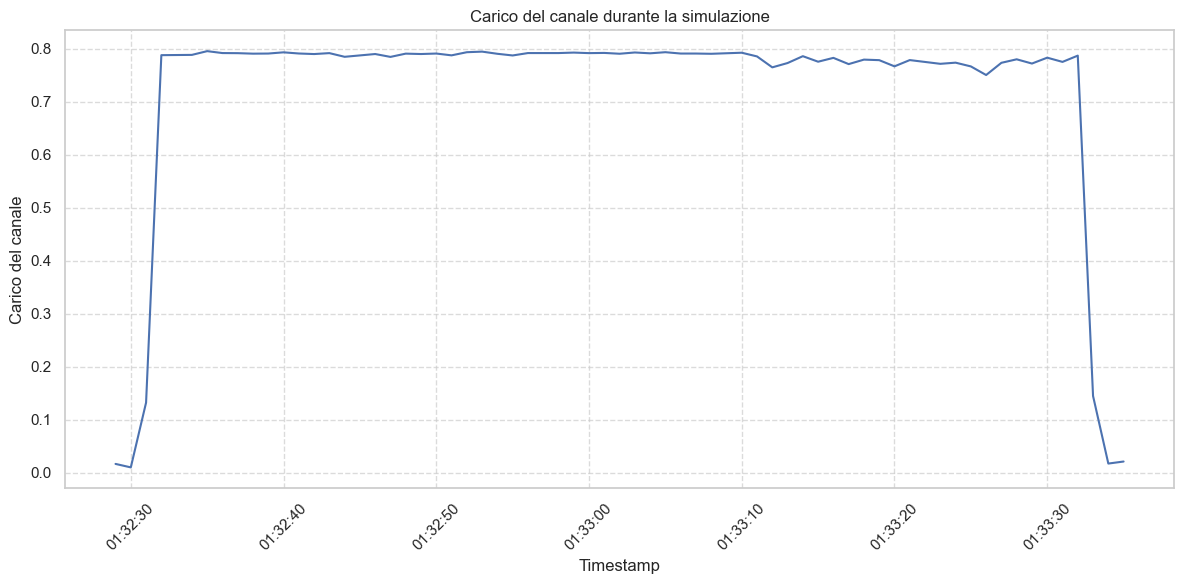
\includegraphics[width=1\textwidth]{t1_c0_load.png}
    \caption{QoS assente e congestione assente (Carico del canale)}
    \label{fig:t1_c0_load}
\end{figure}

\subsection[QoS assente e congestione parziale]{QoS assente e congestione parziale}
L'assenza di politiche di QoS, unito ad un canale parzialmente disturbato da CAM inviati dagli altri due dispositivi (Figura \ref{fig:t1_c1_load}), porta il throughput di ambedue i flussi ad essere simile ma inferiore rispetto al caso precedentemente discusso di circa il 10\%: 3.49 Mbps circa contro 3.13 Mbps qui (Tabella \ref{table:7} e Figure \ref{fig:t1_c1} e \ref{fig:t1_c1_ensemble}).

\begin{table}[h!]
    \centering
    \begin{tabular}{|>{\centering\arraybackslash}p{20em}|>{\centering\arraybackslash}p{7em}|} 
     \hline
     \textbf{} & \textbf{Valori} \\ 
     \hline
     \textbf{Throughput Medio per Stream ID 1} & 3.13 Mbps \\ 
     \hline
     \textbf{Throughput Medio per Stream ID 2} & 3.13 Mbps \\
     \hline
    \end{tabular}
    \caption{Valori medi caso QoS assente e congestione parziale}
    \label{table:7}
\end{table}

\begin{figure}[h!]
    \centering
    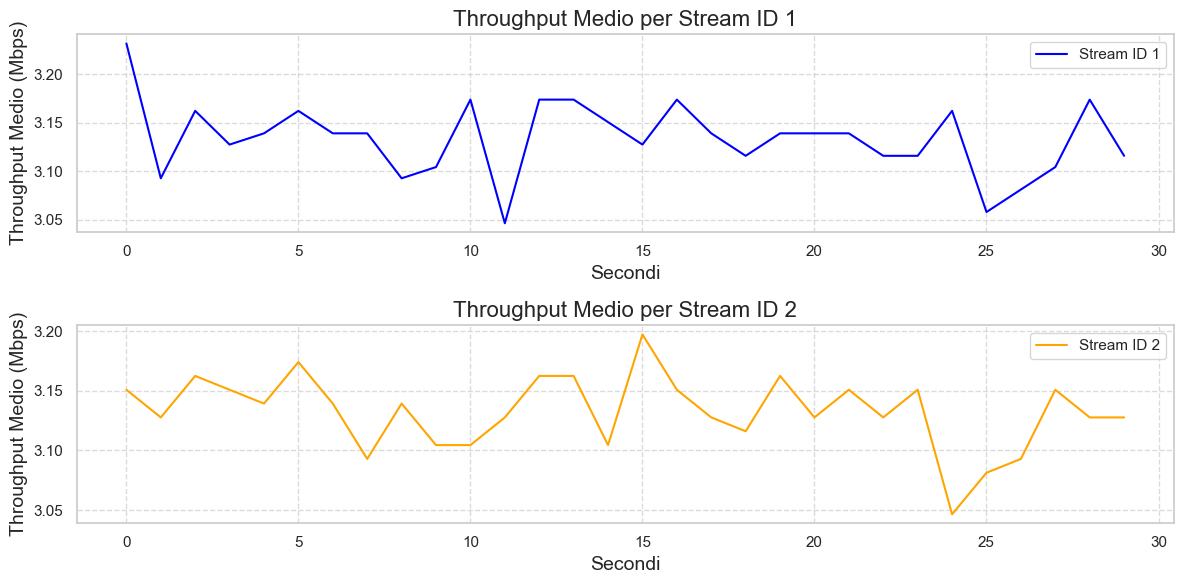
\includegraphics[width=1\textwidth]{t1_c1.png}
    \caption{QoS assente e congestione parziale (Throughput medio)}
    \label{fig:t1_c1}
\end{figure}

\begin{figure}[h!]
    \centering
    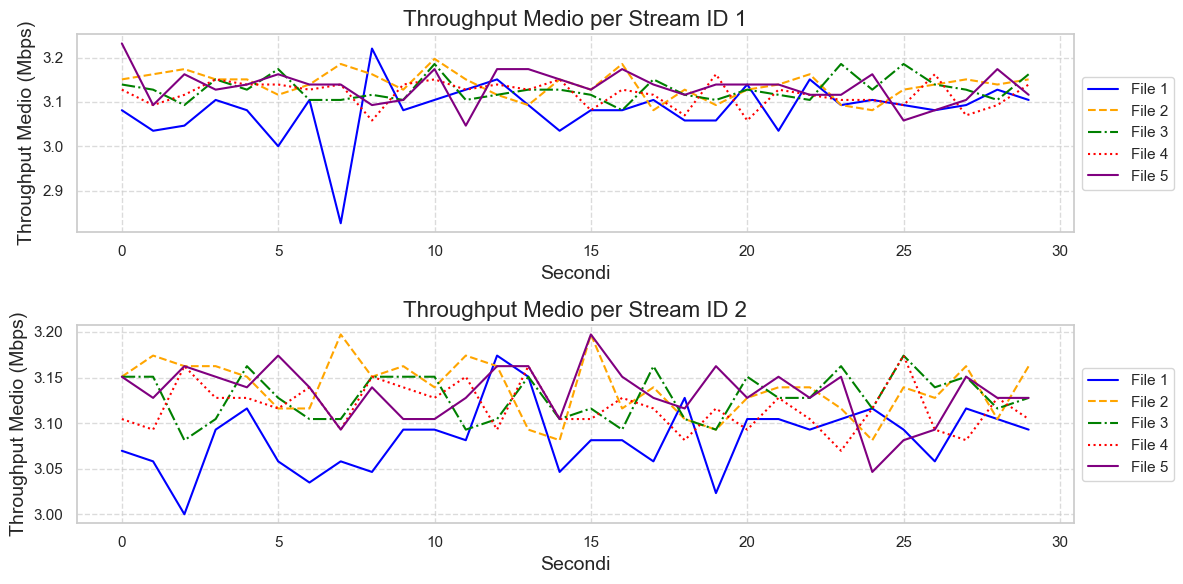
\includegraphics[width=1\textwidth]{t1_c1_ensemble.png}
    \caption{QoS assente e congestione parziale (Grafico ensemble)}
    \label{fig:t1_c1_ensemble}
\end{figure}
\clearpage
\begin{figure}[h!]
    \centering
    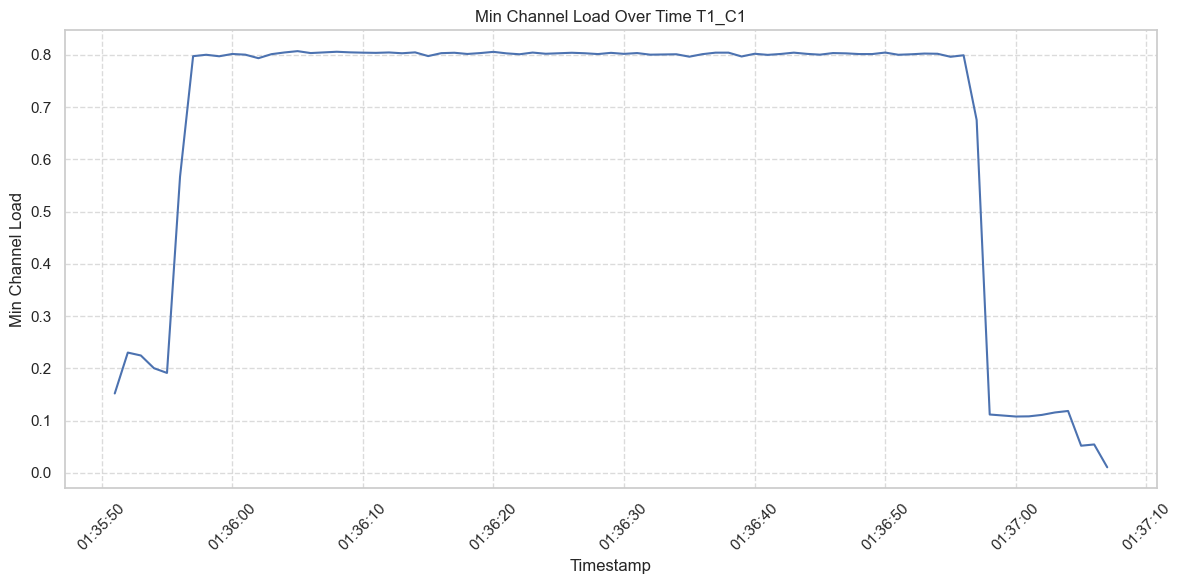
\includegraphics[width=1\textwidth]{t1_c1_load.png}
    \caption{QoS assente e congestione parziale (Carico del canale)}
    \label{fig:t1_c1_load}
\end{figure}

\subsection[QoS assente e congestione totale]{QoS assente e congestione totale}
La completa saturazione del canale qui si fa sentire notevolmente (Figura \ref{fig:t1_c2_load}), in quanto il throughput di ambedue i flussi viene ridotto notevolmente con una minore propensione ad essere stabile rispetto al caso senza congestione: 3.49 Mbps circa contro 1.14 Mbps circa qui (Tabella \ref{table:8} e Figure \ref{fig:t1_c2} e \ref{fig:t1_c2_ensemble}).
\begin{table}[h!]
    \centering
    \begin{tabular}{|>{\centering\arraybackslash}p{20em}|>{\centering\arraybackslash}p{7em}|} 
     \hline
     \textbf{} & \textbf{Valori} \\ 
     \hline
     \textbf{Throughput Medio per Stream ID 1} & 1.14 Mbps \\ 
     \hline
     \textbf{Throughput Medio per Stream ID 2} & 1.19 Mbps \\
     \hline
    \end{tabular}
    \caption{Valori medi caso QoS assente e congestione totale}
    \label{table:8}
\end{table}

\begin{figure}[h!]
    \centering
    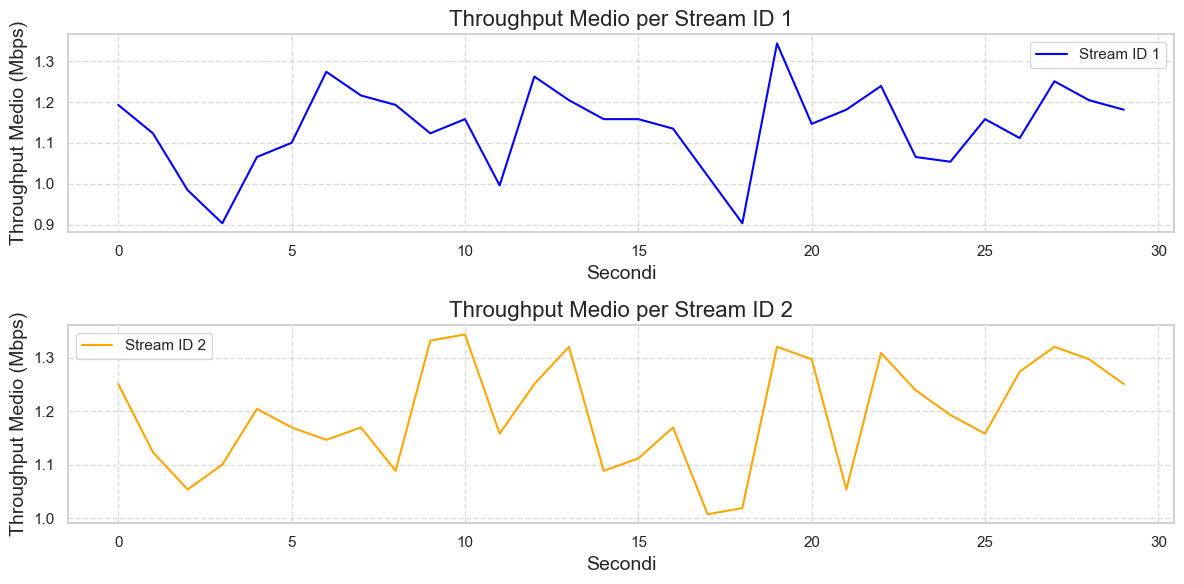
\includegraphics[width=1\textwidth]{t1_c2.png}
    \caption{QoS assente e congestione totale (Throughput medio)}
    \label{fig:t1_c2}
\end{figure}

\begin{figure}[h!]
    \centering
    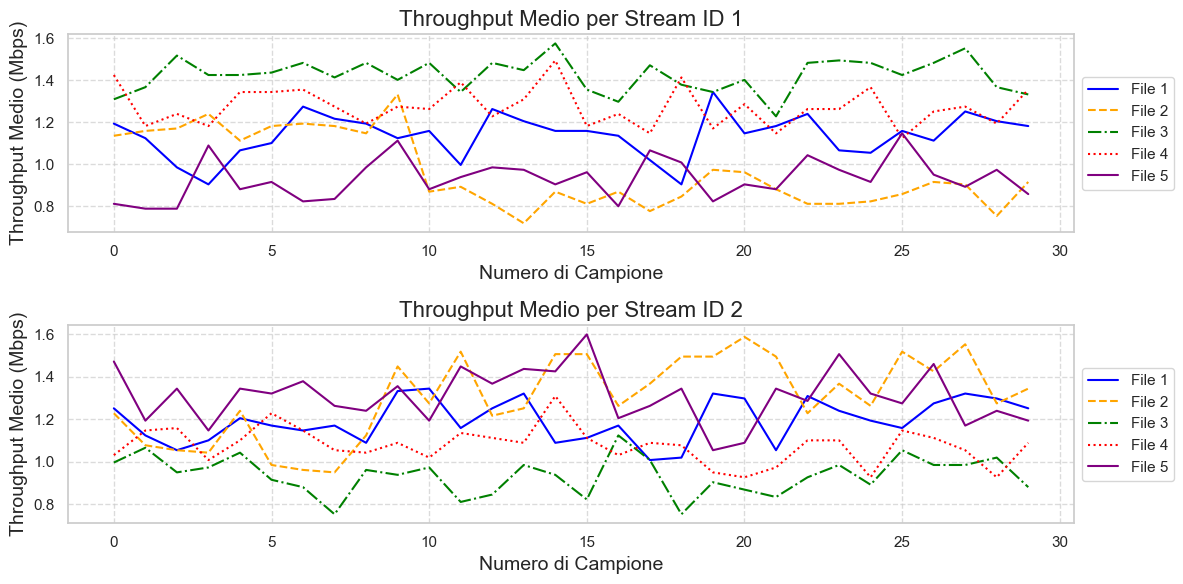
\includegraphics[width=1\textwidth]{t1_c2_ensemble.png}
    \caption{QoS assente e congestione totale (Grafico ensemble)}
    \label{fig:t1_c2_ensemble}
\end{figure}
\clearpage
\begin{figure}[h!]
    \centering
    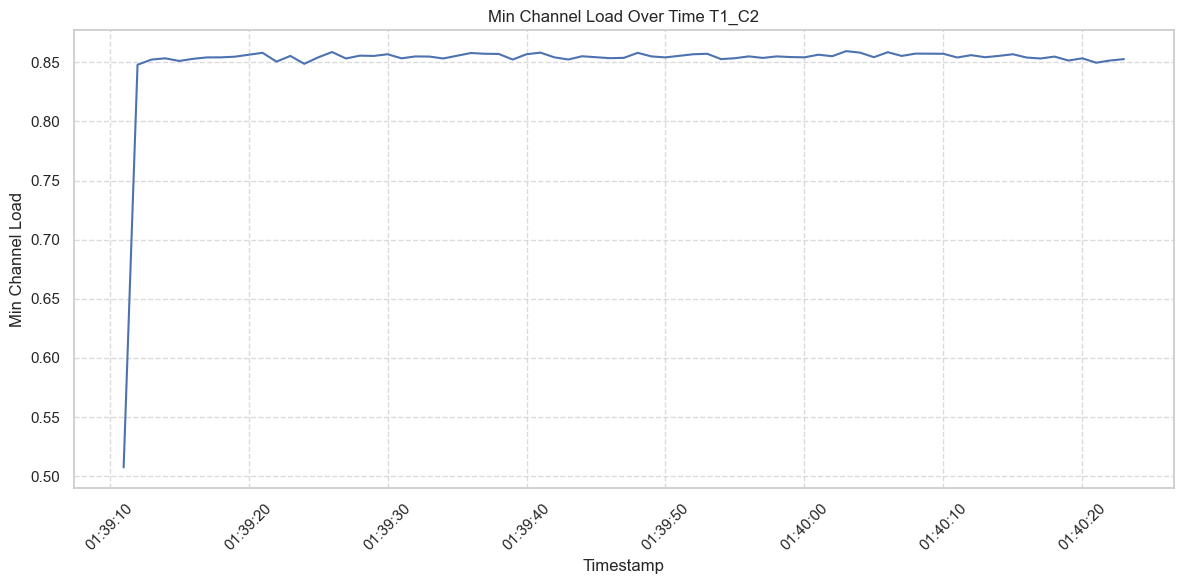
\includegraphics[width=1\textwidth]{t1_c2_load.png}
    \caption{QoS assente e congestione totale (Carico del canale)}
    \label{fig:t1_c2_load}
\end{figure}

\subsection[QoS presente e congestione assente]{QoS presente e congestione assente}
L'inserimento, qui, di politiche di QoS, unito ad un canale quasi completamente vuoto e libero da trasmissioni (Figura \ref{fig:t2_c0_load}), porta il throughput del flusso a priorità maggiore ad sorpaffare completamente l'altro a priorità minore (Tabella \ref{table:9} e Figure \ref{fig:t2_c0} e \ref{fig:t2_c0_ensemble}).

\begin{table}[h!]
    \centering
    \begin{tabular}{|>{\centering\arraybackslash}p{20em}|>{\centering\arraybackslash}p{7em}|} 
     \hline
     \textbf{} & \textbf{Valori} \\ 
     \hline
     \textbf{Throughput Medio per Stream ID 1} & 7.96 Mbps \\ 
     \hline
     \textbf{Throughput Medio per Stream ID 2} & 0.61 Mbps \\
     \hline
    \end{tabular}
    \caption{Valori medi caso QoS presente e congestione assente}
    \label{table:9}
\end{table}

\begin{figure}[h!]
    \centering
    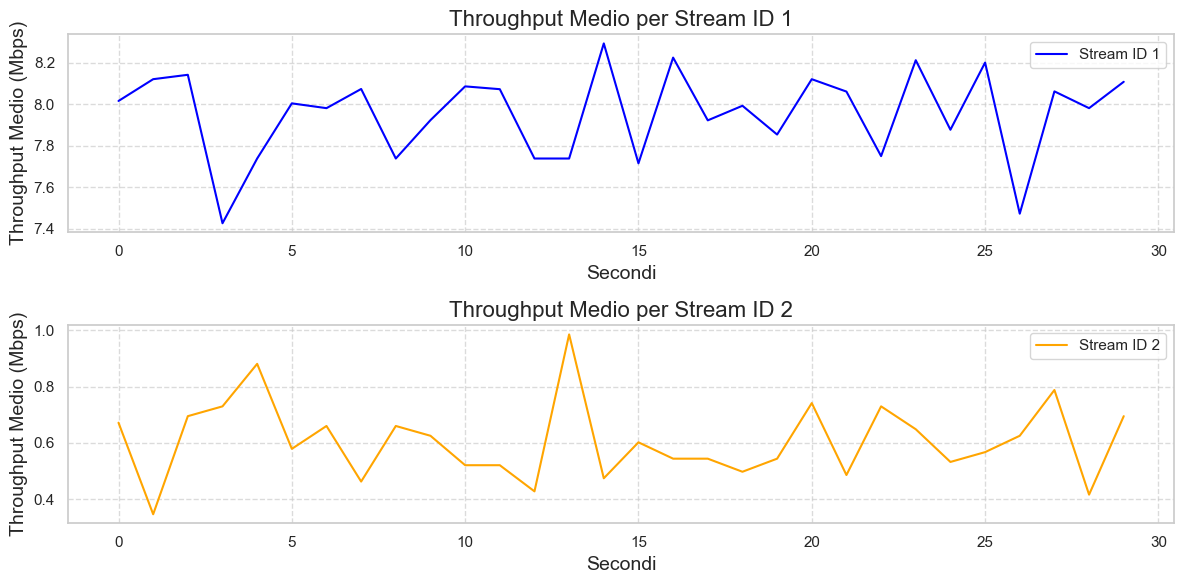
\includegraphics[width=1\textwidth]{t2_c0.png}
    \caption{QoS presente e congestione assente (Throughput medio)}
    \label{fig:t2_c0}
\end{figure}

\begin{figure}[h!]
    \centering
    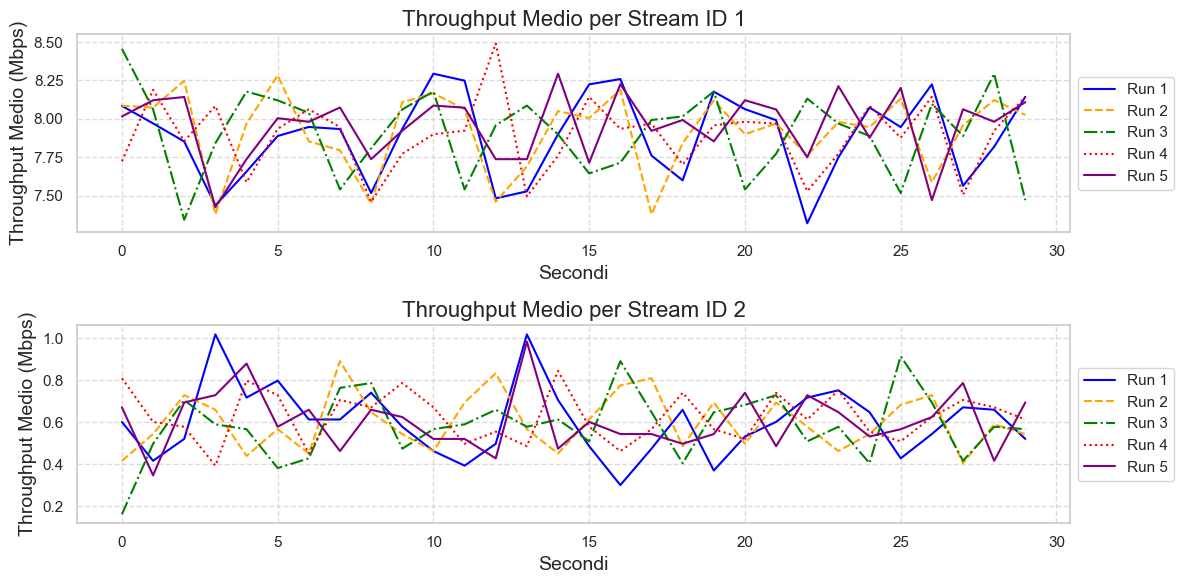
\includegraphics[width=1\textwidth]{t2_c0_ensemble.png}
    \caption{QoS presente e congestione assente (Grafico ensemble)}
    \label{fig:t2_c0_ensemble}
\end{figure}
\clearpage
\begin{figure}[h!]
    \centering
    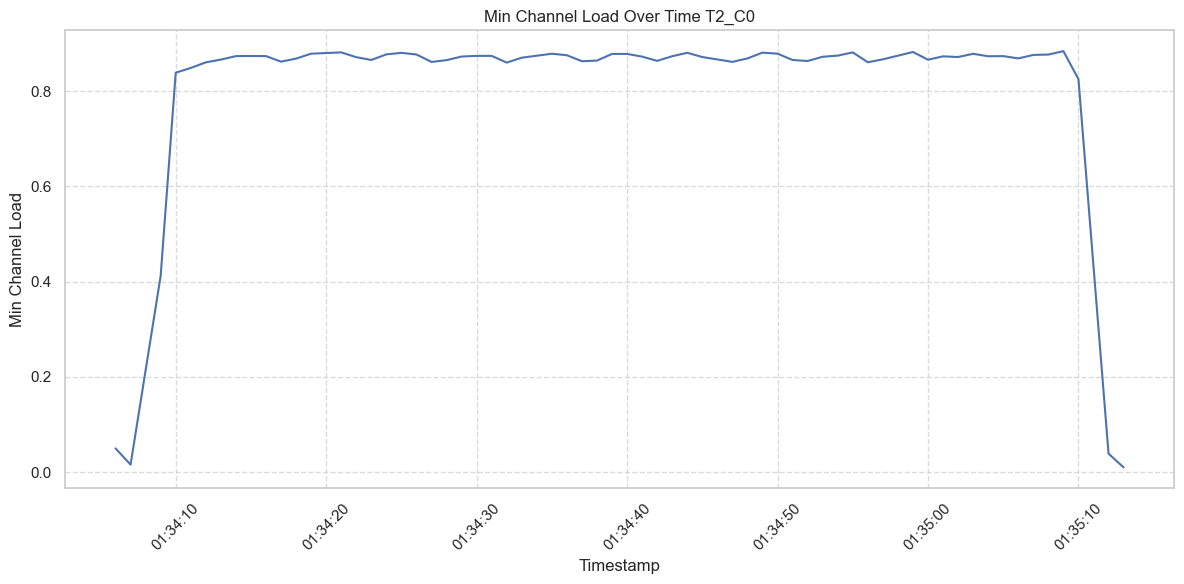
\includegraphics[width=1\textwidth]{t2_c0_load.png}
    \caption{QoS presente e congestione assente (Carico del canale)}
    \label{fig:t2_c0_load}
\end{figure}

\subsection[QoS presente e congestione parziale]{QoS presente e congestione parziale}
\begin{table}[h!]
    \centering
    \begin{tabular}{|>{\centering\arraybackslash}p{20em}|>{\centering\arraybackslash}p{7em}|} 
     \hline
     \textbf{} & \textbf{Valori} \\ 
     \hline
     \textbf{Throughput Medio per Stream ID 1} & 6.73 Mbps \\ 
     \hline
     \textbf{Throughput Medio per Stream ID 2} & 0.77 Mbps \\
     \hline
    \end{tabular}
    \caption{Valori medi caso QoS presente e congestione parziale}
    \label{table:10}
\end{table}

\begin{figure}[h!]
    \centering
    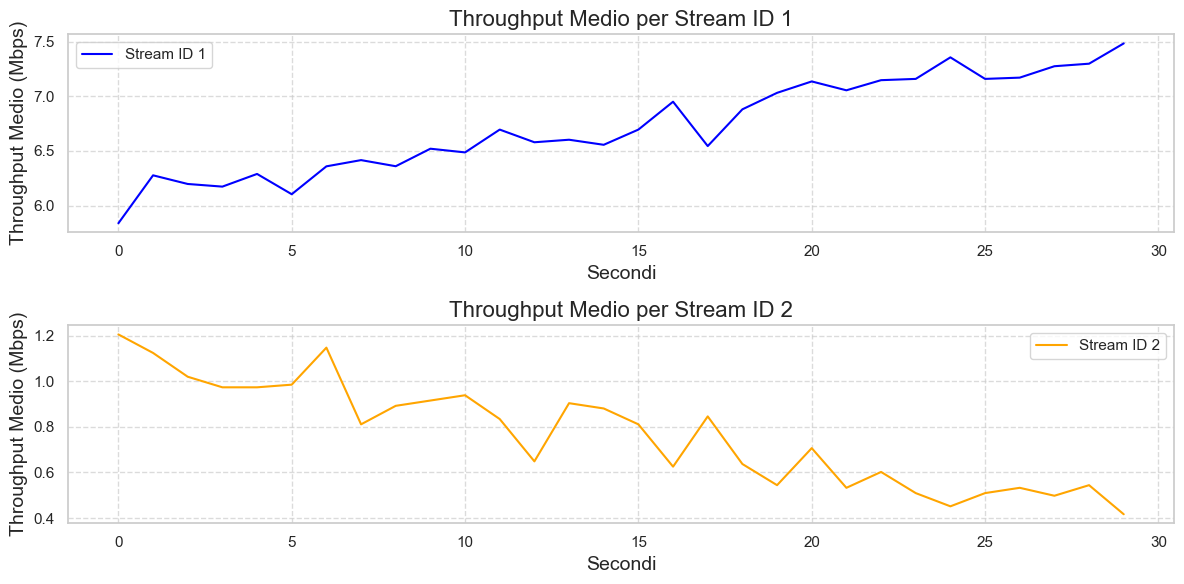
\includegraphics[width=1\textwidth]{t2_c1.png}
    \caption{QoS presente e congestione parziale (Throughput medio)}
    \label{fig:t2_c1}
\end{figure}

\begin{figure}[h!]
    \centering
    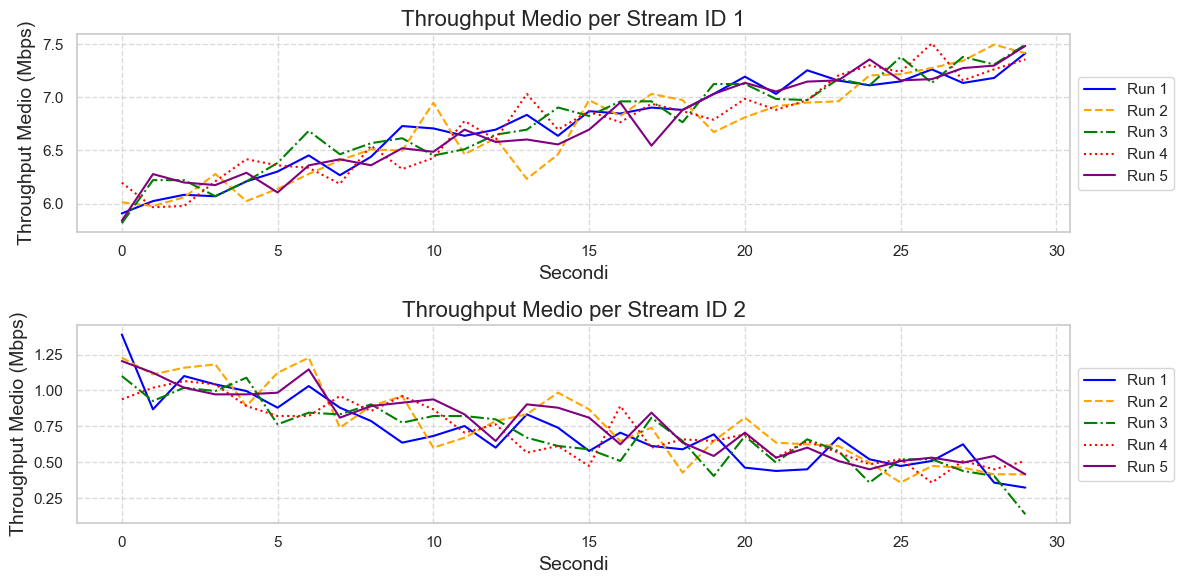
\includegraphics[width=1\textwidth]{t2_c1_ensemble.png}
    \caption{QoS presente e congestione parziale (Grafico ensemble)}
    \label{fig:t2_c1_ensemble}
\end{figure}
\clearpage
\begin{figure}[h!]
    \centering
    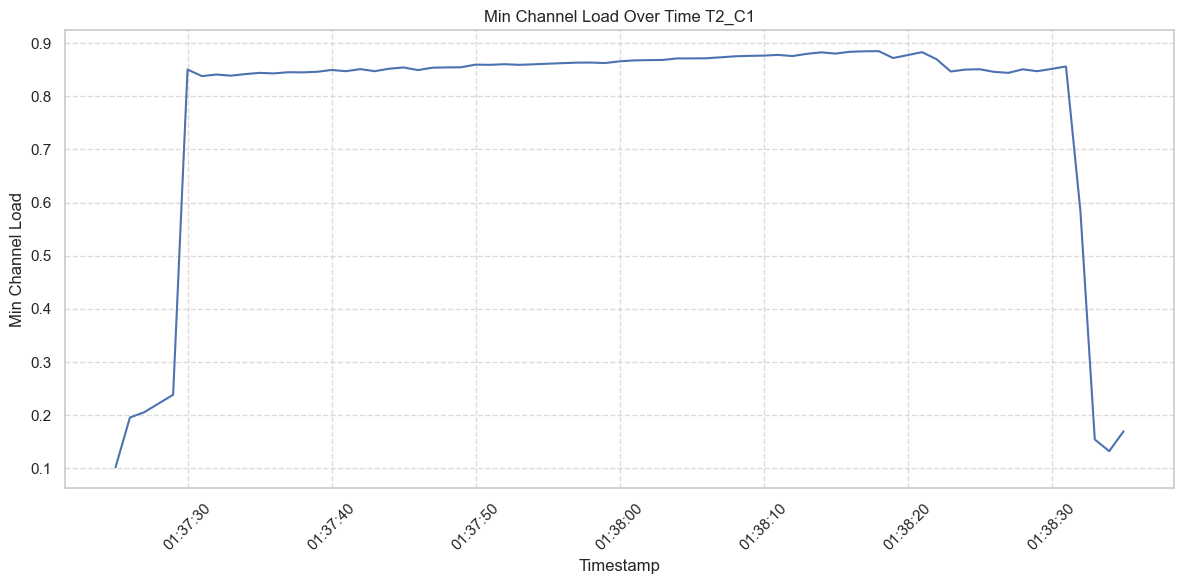
\includegraphics[width=1\textwidth]{t2_c1_load.png}
    \caption{QoS presente e congestione parziale (Carico del canale)}
    \label{fig:t2_c1_load}
\end{figure}

\subsection[QoS presente e congestione totale]{QoS presente e congestione totale}
La completa saturazione del canale qui si fa sentire notevolmente (Figura \ref{fig:t2_c2_load}), in quanto il throughput di ambedue i flussi viene ridotto notevolmente con un inoltre minore propensione ad essere stabile rispetto al caso senza congestione. (Tabella \ref{table:11} e Figure \ref{fig:t2_c2} e \ref{fig:t2_c2_ensemble}). L'applicazione di politiche di QoS porta, naturalmente, ad un throughput medio maggiore del flusso a priorità maggiore.

\begin{table}[h!]
    \centering
    \begin{tabular}{|>{\centering\arraybackslash}p{20em}|>{\centering\arraybackslash}p{7em}|} 
     \hline
     \textbf{} & \textbf{Valori} \\ 
     \hline
     \textbf{Throughput Medio per Stream ID 1} & 6.19 Mbps \\ 
     \hline
     \textbf{Throughput Medio per Stream ID 2} & 0.30 Mbps \\
     \hline
    \end{tabular}
    \caption{Valori medi caso QoS presente e congestione totale}
    \label{table:11}
\end{table}

\begin{figure}[h!]
    \centering
    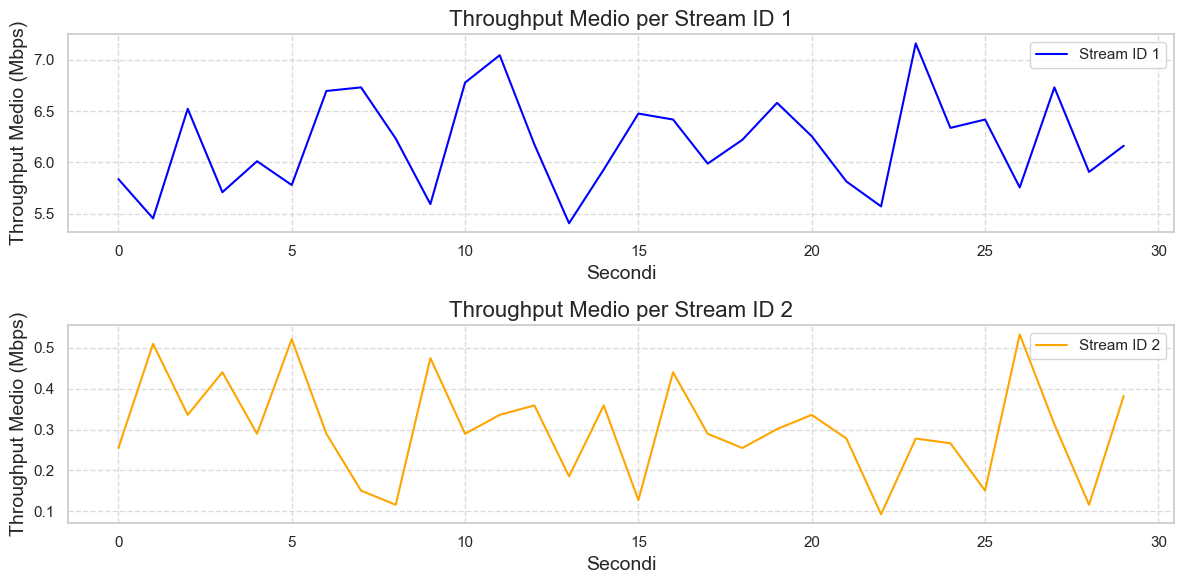
\includegraphics[width=1\textwidth]{t2_c2.png}
    \caption{QoS presente e congestione totale (Throughput medio)}
    \label{fig:t2_c2}
\end{figure}

\begin{figure}[h!]
    \centering
    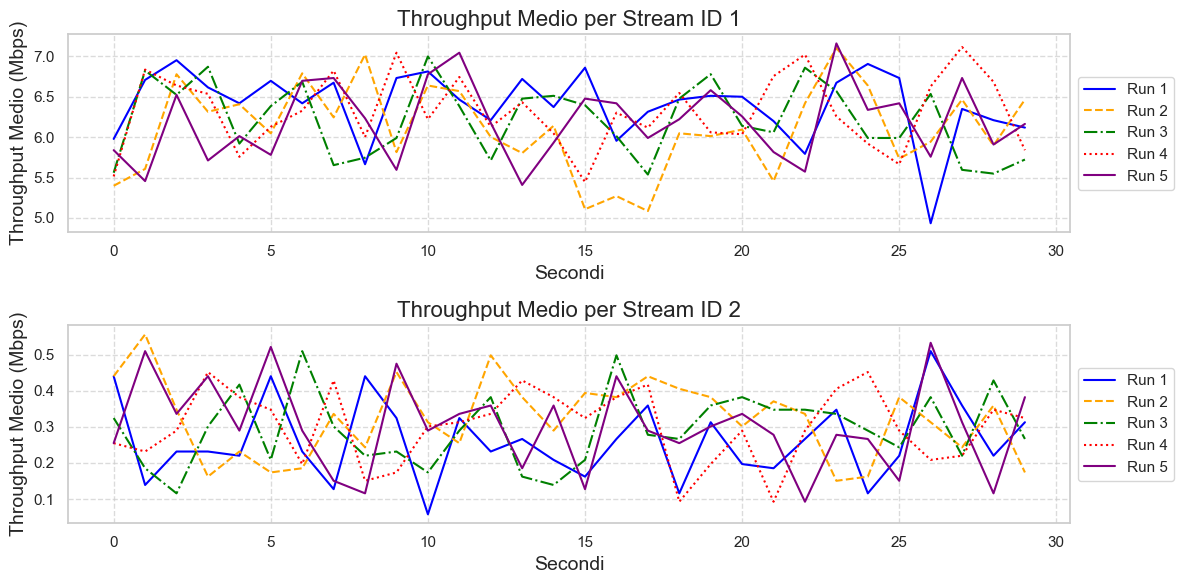
\includegraphics[width=1\textwidth]{t2_c2_ensemble.png}
    \caption{QoS presente e congestione totale (Grafico ensemble)}
    \label{fig:t2_c2_ensemble}
\end{figure}
\clearpage
\begin{figure}[h!]
    \centering
    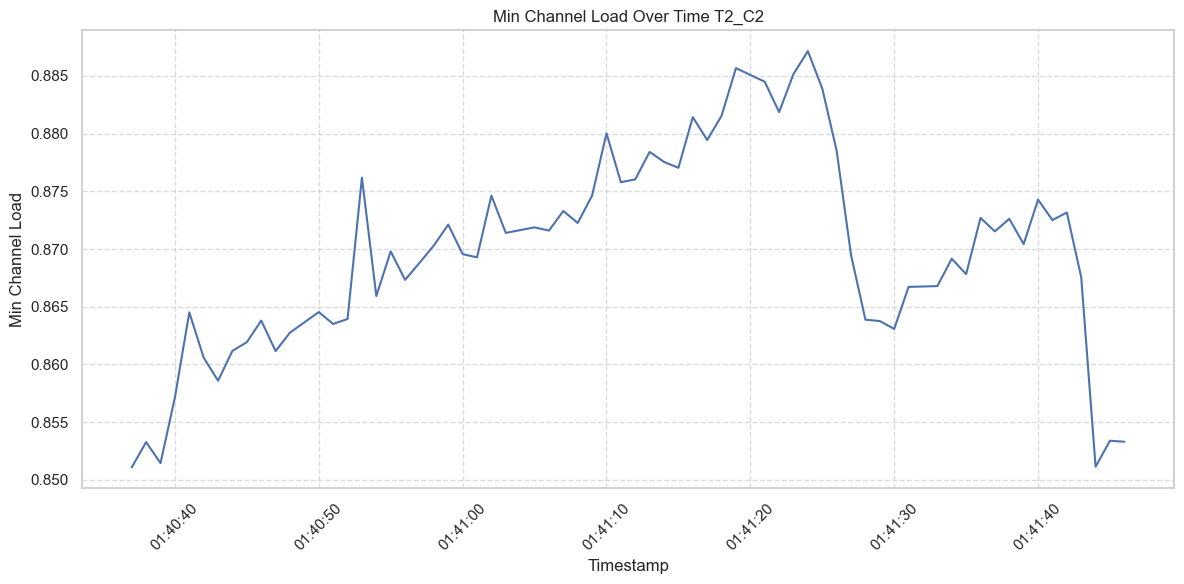
\includegraphics[width=1\textwidth]{t2_c2_load.png}
    \caption{QoS presente e congestione totale (Carico del canale)}
    \label{fig:t2_c2_load}
\end{figure}
\section{Test 2}

\section{Lost packets}